\chapter{Preliminaries \label{chap:Preliminaries}}



In this chapter we will give a brief description description about transport processes in quantum dots (QDs). This will lead us to talk discuss the Anderson model and the Kondo effect,which are key ingredients in the objective of this project . 

%-------------------------------------------------------------
%Here goes the introduction of transport between quantum dots. stil need to add important considerations like the smooth varying DOS. Not so discrete. 
%Assumption: 
%   1-Only the level immediately at the bottom of the fermi       level is considered
\section{Transport in Quantum Dots (QDs)}
% --------------Figure-------------------------
\begin{figure}[hbt]
    \centering
    \subfloat[\label{QD-figuresA}\label{QD-figures}]{\includegraphics[scale=0.3]{IMAGES/Preliminars/VerticalQD.png}}\hspace{6mm}
    \subfloat[\label{QD-figuresB}]{\includegraphics[scale=0.4]{IMAGES/Preliminars/QD-horizontal.png}}
    \caption{ a) Vertical quantum dot.  b)Atomic force microscopy
    picture of two coupled lateral QDs (bright central circles). Gates 1 and 2 act as drain and source voltage. A negative
    voltage is applied at gates $A$,$B$ to allow the formation of the droplets inside the free space in the 2D electron gas. \protect\Source{\cite{holleitner_probing_2002}} }
\end{figure}

Quantum mechanical effects are visible when the system size is of the order of the de Broglie wavelength \citep[(1.1)]{bimberg_quantum_1999}
\[
\lambda_{f}=\frac{h}{\sqrt{3m_{\mathsf{eff}}k_{B}T}}
\]
 where $m_{\mathsf{eff}}$ is the electron effective mass in the crystal.
Since $m_{\mathsf{eff}}$ can be much smaller than the free electron mass in some semiconducting materials, size quantization effects can be observed at system of sizes $\sim100\mbox{nm}$ \citep[2.1]{sindel_numerical_2005}. A $0$D quantum system is a device confined in the three spacial dimensions up to this length-scale. This type of devices receive the name of quantum dots (QD). 

\begin{figure}[tb]
    \centering
    \includegraphics[scale=0.5]{IMAGES/Preliminars/specDot.png}
    \caption{Pictorial representation of the Density of States of a QD. The gate potential $V_G$ can be tuned to change the fermi energy of the dot.  \protect\Source{By the author} }
    \label{fig:specDots}
\end{figure}


\begin{figure}[t]
     \centering
    
     \subfloat[ \label{fig:QD-transport}]{\includegraphics[scale=0.7]{IMAGES/Preliminars/QD-Transport.png}}
    \subfloat[\label{fig:QD-Blockade}]{\includegraphics[scale=0.3]{IMAGES/Preliminars/QD-Blockade1.png}}
     \caption{ a) Representation of transport through QD. The red curve represents the hybridized energy level. The gate voltage tunes this level. In the case represented, the energy level is in the middle of the drain and source voltages allowing transport between the leads. b) Charging diagram of a quantum dot. Differential conductance dependence over the gate voltage $V_G$ and the source-drain voltage $(V_{SD}=V_{S}-V_{D} )$. Coulomb blockade occurs at the diamond-shaped regions with zero conductance. At these regions the number of electrons is constant and increases $1$ by $1$ when the gate voltage is scaled up.  \protect\Source{a) By the Author , b) Adapted from \cite{sindel_numerical_2005}  }}
\end{figure}

  Nowadays, QDs can be manufactured with different substracts, geometries and  and orientations \citep{bimberg_quantum_1999}. They can be merged in structures like double quantum dots (\ref{QD-figuresA}) or can even be built out vertical to the base 2D-electron gas (\ref{QD-figuresB}). The precise experimental control over these devices allows to design atom-like structures with controllable energy levels. This has important applications on laser physics and in the implementation of single electron transistors. 
  % According to their orientation with respect to the based 2D-plane  two main types of QDs can be distinguished : Vertical (Figure \ref{QD-figuresA}) and lateral (Figure \ref{QD-figuresB}) QDs. 


  Usually quantum dots have $3$-main gates. Two of them are the Drain $V_D$ and source $V_S$ voltages used to control the electric gradient through the QD. The third one is the gate voltage $V_G$ which allows to control with high precision the number of electrons inside the dot. 

   Ideally, the energy spectrum of a QD is a discrete set of energy levels resembling the spectrum of an atom.  When the QD is connected to metallic leads these energy levels hybridized with respect to a broadening parameter $\Gamma$ which increases as the square of the source-drain voltage $V_{SD}$ 
\begin{equation}
    \Gamma \propto \pi \Vert V_{SD} \Vert^2
\end{equation}

in a flat band approximation. This broadening is depicted in \ref{fig:specDots}. Ideally, $\Gamma \ll \Delta E$ is smaller enough such that the energy levels do not overlap each other. 

It is possible to execute transport measurements through a QD attached to two leads, source and drain (See \ref{fig:QD-transport}) . Each lead will have a characteristic gate voltage $V_S$ (Left lead) and $V_D$ (Right lead). An electron can pass from the source to the drain if there is an energy level in the middle of the two voltages, just as in \ref{fig:QD-transport}. If this condition is not satisfied,  the dot enters into a coulomb blockade region without  electron transport between both leads as can be observed in \ref{fig:QD-Blockade}. Inside the coulomb blockade regions described (black diamonds) the number of electrons is constant. When increasing $V_G$ a single electron enters into the dot each time the system makes a transition between blockade regions. Since all of these effects can be controlled precisely with the gate voltage, the system described is indeed a single electron transistor (SET).  






% Indeed we can model an ideal single-electron QD as a quantum well
% with a negative constant potential inside the dot . For example an
% spherical quantum dot with radius $R$ will take the following Schr�dinger
% Hamiltonian 

% \[
% H\Psi(r)=\left(\frac{\hbar^{2}}{2m^{*}}\nabla^{2}+V(r)\right)\Psi(r)\ ,\ \textrm{with }V(r)=\begin{cases}
% -V_{0} & r<R\\
% 0 & r\geq R
% \end{cases}.
% \]


% The 
% the energy level spacing is  \citep[Equation (5.44)]{bimberg_quantum_1999}

% \[
% \delta E\propto\frac{1}{R^{2}}.
% \]



%------------------------------------------------------------
\section{The Anderson Model}
% The key ingredient in the Kondo phenomena is the presence of magnetic impurities whose states are hybridized to conduction electron in the metal. To study this idea the physics Nobel prize winner Philip Anderson created a model that simulated the quantum interaction between the impurity and the conduction band \citep{anderson_localized_1961}. The Anderson Model can be applied to different problems. In this thesis we are mainly interested in the study of artificially manufacture impurities better known as quantum dots.   

 %Here the study of the  magnetic impurities in metals responsible for the Kondo effect, as well as artificial impurities like quantum dots. 
 The Anderson model is used to describe quantum impurity systems where Coulomb repulsions and strongly correlated phenomena are dominant \citep{anderson_localized_1961}. A quantum dot attached to a metallic lead is basically an artificial impurity that can be experimentally designed, modified and manipulated. Hence QDs are is the perfect type of structure to probe the of the physics behind   Anderson's ideas.  

 Due to the small confinement space inside these dots, the coulomb repulsion is relevant. However, it is usually impossible to provide a complete analytical description of these kind of systems due to the high correlations generated by this factor. Instead, we can obtain an overall description of the transport through the impurity by neglecting this coulomb repulsion. This will allow us to obtain some analytic intuition of the models  before adventuring with long-lasting numerical simulations of interacting models. During this thesis, we will consider these two regimes as follows
\begin{itemize}
    \item \textbf{Non-interacting systems:} Coulomb repulsion is not relevant . In this case, spin-$\uparrow$ and spin-$\dw$ channels are independent which simplifies many of the procedures. They can be described analytically through the ballistic transport approach. 

    \item \textbf{Interacting systems:} The coulomb repulsion is relevant. The repulsion factor will be defined by the factor $U$ which will take a fix value during the entire project. In this case, spin-$\uparrow$ and spin-$\dw$ channels are not independent since the coulomb repulsion limits the number of particles inside each dot. We will use the Numerical Renormalization Group to treat this case. The intuition acquired from non-interacting systems will help us to select the input parameters of the algorithm.  
\end{itemize}


%The Anderson model takes in account both regimes and  the only difference in each case will be the value of $U$ parameter ($U=0$ non-interacting , $U>0$ interacting). 

To build the Anderson model first consider that we have a QD (impurity) coupled to the conduction band of a metallic lead. We will define a coulomb repulsion factor $U$ which will be set to $0$ if the system is non-interacting . Using the Hunds rules we know that the energy levels inside the dot should be filled from lower to higher energies with two electrons with different spin at each state. Each pair of electrons will interact magnetically and electrically. In addition, there is and energy term associated to each electron and a Zeeman splitting factor in case a $\hat{z}$-directed magnetic field $B$ is placed.  Considering these interactions we can obtain a very general expression in second quantization for the QD Hamiltonian
of the form \citep[(3.2)]{sindel_numerical_2005}

\[
H_{d}=\sum_{i\sigma}\epsilon_{di}d_{i\sigma}^{\dagger}d_{i\sigma}+\sum_{i}U_{i}\hat{n}_{i\uparrow}\hat{n}_{i\downarrow}+\sum_{\sigma\sigma',i\neq j}U_{ij}\hat{n}_{i\sigma}\hat{n}_{j\sigma'}-\mu_{B}gB\sum_{i}S_{i}^{z}+J\sum_{i\neq j}\mathbf{S}_{i}\cdot\mathbf{S}_{j}.
\]


Where $\sigma\in\{\uparrow,\downarrow\}$, $d_{i\sigma}^{\dagger}\left(d_{i\sigma}\right)$
is the dot creation(annihilation) operator,$\hat{n}_{i\sigma}:=d_{i\sigma}^{\dagger}d_{i\sigma}$
is the particle number, $\mathbf{S}_{i}$ is the spin-vector, $\epsilon_{di}$
is the energy of the $i^{\mbox{th}}$-level in the dot, $U_{i}$ is
the coulomb repulsion between electrons in the same energy level $i$,
$U_{ij}$ is the coulomb interaction between electrons in different
levels (And therefore smaller than $U_{i}$), \textbf{$B$} is an
applied magnetic field in the $\hat{z}$-direction and $J$ is the
term representing the Zeeman splitting. 

At low temperatures, the quantum interactions occur only with the level closest to the Fermi energy. This allows us to make the single-level approximation, neglecting the other energy levels. This assumption reduces the complexity of the dot Hamiltonian to \\


\begin{equation}
    H_{d}=\sum_{\sigma}\epsilon_{d}d_{\sigma}^{\dagger}d_{\sigma}+U\hat{n}_{\uparrow}\hat{n}_{\downarrow}-\mu_{B}gBS^{z}. \label{eq:hdot}
\end{equation}

Besides to the dot Hamiltonian, we need to consider the energy of the electrons in the lead $H_{lead}$ and the dot-lead interaction $H_{int}$. We can model  the conduction band of the lead as a $2D$ electron gas with the following Bloch Hamiltonian
\begin{equation}
H_{lead}  =  \sum_{\mathbf{k}\sigma l}\epsilon_{\mathbf{k}l}c_{\mathbf{k}\sigma l}^{\dagger}c_{\mathbf{k}\sigma l}. 
\end{equation}

where $\mathbf{k}$ represents the possible crystal momentums in the
leads, $l\in\{S,D\}$, $c_{\mathbf{k}\sigma l}^{\dagger}(c_{\mathbf{k}\sigma l})$
creates(annihilates) an electron with momentum $\mathbf{k}$ and spin
$\sigma$ in the lead $l$, $\epsilon_{\mathbf{k}l}$ is the energy
of the electron in the leads. 

The interaction between the dot and the leads is then given by 
\begin{equation}
H_{int} = \sum_{\mathbf{k}\sigma l}V_{\mathbf{k}l}c_{\mathbf{k}\sigma l}^{\dagger}d_{\sigma}+V_{\mathbf{k}l}^{*}d_{\sigma}^{\dagger}c_{\mathbf{k}\sigma l},
\end{equation}
%\begin{eqnarray*}
%H_{lead} & = & \sum_{\mathbf{k}\sigma l}\epsilon_{\mathbf{k}l}c_{\mathbf{k}\sigma l}^{\dagger}c_{\mathbf{k}\sigma l}\\

%\end{eqnarray*}

where $V_{\mathbf{k}l}$ is a hopping exchange
term between the leads and the QD. 


The sum of all of these three interactions is receives the name of Anderson Model. 
\begin{eqnarray}
H & = & H_{d}+H_{lead}+H_{int}\nonumber \\
 & = & \sum_{\sigma}\epsilon_{d}d_{\sigma}^{\dagger}d_{\sigma}+U\hat{n}_{\uparrow}\hat{n}_{\downarrow}-\mu_{B}gBS^{z}+\sum_{\mathbf{k}\sigma l}\epsilon_{\mathbf{k}l}c_{\mathbf{k}\sigma l}^{\dagger}c_{\mathbf{k}\sigma l}+\sum_{\mathbf{k}\sigma l}V_{\mathbf{k}l}c_{k\sigma l}^{\dagger}d_{\sigma}+V_{\mathbf{k}l}^{*}d_{\sigma}^{\dagger}c_{\mathbf{k}\sigma l}.\label{eq:Anderson}
\end{eqnarray}

For this project, we will make two extra changes to the Anderson model. Using the anti-commutation properties of the fermion operators

% \begin{equation}
% H=H_{d}+H_{lead}+H_{int}=\sum_{\sigma}\epsilon_{d}d_{\sigma}^{\dagger}d_{\sigma}+U\hat{n}_{\uparrow}\hat{n}_{\downarrow}+\sum_{\mathbf{k}\sigma l}\epsilon_{\mathbf{k}l}c_{\mathbf{k}\sigma l}^{\dagger}c_{\mathbf{k}\sigma l}+V_{\mathbf{k}l}c_{\mathbf{k}\sigma l}^{\dagger}d_{\sigma}+V_{\mathbf{k}l}^{*}d_{\sigma}^{\dagger}c_{\mathbf{k}\sigma l}.\label{eq:hamB0}
% \end{equation}
\[
\left\{ d_{\sigma}^{\dagger},d_{\sigma'}\right\} =\delta_{\sigma\sigma'}\ ,\ \left\{ d_{\sigma}^{\dagger},d_{\sigma'}^{\dagger}\right\} =\left\{ d_{\sigma},d_{\sigma'}\right\} =0
\]
we get


\begin{eqnarray*}
\left(d_{\up}^{\dagger}d_{\up}+d_{\down}^{\dagger}d_{\down}-1\right){}^{2} & = & \sum_{\sigma}\left(d_{\sigma}^{\dagger}d_{\sigma}\right)^{2}-2\sum_{\sigma}d_{\sigma}^{\dagger}d_{\sigma}+2d_{\up}^{\dagger}d_{\up}d_{\down}^{\dagger}d_{\down}-1\\
 & = & 2d_{\up}^{\dagger}d_{\up}d_{\down}^{\dagger}d_{\down}-\sum_{\sigma}d_{\sigma}^{\dagger}d_{\sigma}-1.
\end{eqnarray*}

Replacing this in \eqref{eq:hdot} we obtain a  nice spin-symmetric form of the dot hamiltonian

\begin{equation}
    \left(\epsilon_{d}+\frac{U}{2}\right)d_{\sigma}^{\dagger}d_{\sigma}+\frac{U}{2}(d_{\sigma}^{\dagger}d_{\sigma}-1)^{2}-\mu_{B}gBS^{z}. 
    \label{eq:hdot2}
\end{equation}

In addition, it is possible to do a linear transform to the lead opperators 
\begin{equation}
    \frac{1}{\sqrt{V_{S}^{2}+V_{R}^{2}}}\left[\begin{array}{cc}
V_{S} & V_{R}\\
-V_{R} & V_{S}
\end{array}\right]\left[\begin{array}{c}
c_{\mathbf{k}\sigma S}\\
c_{\mathbf{k}\sigma D}
\end{array}\right]=\left[\begin{array}{c}
c_{\mathbf{k}\sigma+}\\
c_{\mathbf{k}\sigma-}
\end{array}\right]
\end{equation}
After the transformation the operator will be decoupled from the dot hamiltonian $c_{\mathbf{k}\sigma-}$ . This implies that we can suppose that the  \textbf{dot is coupled wit just one lead}. During the rest of the thesis we will maintain this convention. 


%------------------------------------------------------------
\section{The Kondo Effect \label{sec:Kondo} }


\begin{figure}[t]
     \centering
    
     \subfloat[ \label{fig:KondoTemp}]{\includegraphics[scale=0.6]{IMAGES/Preliminars/KondoTemp.png}}
    \subfloat[\label{fig:KondoKloud}]{\includegraphics[scale=1.3]{IMAGES/Preliminars/kondoCloud.png}}
     \caption{ a) Resistivity minimum near the Kondo temperature $T_k$. b) Kondo cloud formed by a singlet grouped around the impurity divided in spin-$\up$,spin-$\dw$ regions.   \protect\Source{a) \cite{Kondo_deBoer1934} , b) \cite{Ternes_2008}  }}
\end{figure}


The Kondo effect is one of the biggest condensed matter problems in the 20th century. There was an uncountable number of experimental and theoretical physicist that contributed to this problem . The most reknown are probably the physicists Jacques Friedel, Jun Kondo and the two nobel prizes Philip Anderson and Kenneth Wilson \citep{hewson_kondo_1997}. 

The history of the Kondo effect began in the early 1930s. By that time it was known that the resistivity of a metal is regulated by different scattering interactions against lattice phonon vibrations $\rho_{phonon} \sim T^5$, other electrons $\sim T^2$ and static impurities, which is temperature independent. The form of these contribution clearly implies that the resistivity should decay uniformly with a decreasing temperature. Nevertheless, some groundbreaking experiments revealed the observation of a resistance minimum in some metals at temperatures lower than $10K$ \cite{Kondo_deBoer1934} (See \ref{fig:KondoTemp} ). 

This phenomenon intrigued the scientific community for the following decades until the year 1964 when the physicist  Jun Kondo gave the first convincing solution to this puzzle. Kondo attributed the phenomenon to the scattering of the electrons due to the spin-interaction with a small concentration of magnetic impurities in the metal. To describe it he proposed the following interaction Hamiltonian

%\begin{equation}
%H_K = H_l + 2J\hat{\textbf{S}}\cdot \hat{\textbf{s}}_0
%\end{equation}

\begin{align}
H_K &= 2J\hat{\textbf{S}}\cdot \hat{\textbf{s}} \\
&=  J (2S_z s_z + S_+s_- +S_-s_+)
\end{align}
with $S_\pm = S_x \pm iS_y$. The hamiltonian $H_K$ which is better known as the Kondo s-d model describes the spin interaction between the spin of the impurity $\hat{\textbf{S}}$ and the spin of the particles in the metal $\hat{\textbf{s}}$.
% These particles can be described with the Hamiltonian 

%\begin{equation}
%H_{M}  =  \sum_{\mathbf{k}\sigma }\epsilon_{\mathbf{k}}c_{\mathbf{k}\sigma}^{\dagger}c_{\mathbf{k}\sigma },
%\end{equation}

%such that $c_{\mathbf{k}\sigma }$ is the creation operator of a particle with spin-$\sigma$ and momentum $k$. The spin operators can be also written in terms of these as
%\begin{align}
%    s_z &= \sum_{\mathbf{k},\mathbf{k'}} c_{\mathbf{k}\up}^{\dagger}c_{\mathbf{k'}\up} - c_{\mathbf{k}\dw}^{\dagger}c_{\mathbf{k'}\dw} \\
%    s_+ &= \sum_{\mathbf{k},\mathbf{k'}} c_{\mathbf{k}\up}^{\dagger}c_{\mathbf{k'}\dw}  \\
%    s_- &= \sum_{\mathbf{k},\mathbf{k'}} c_{\mathbf{k}\dw}^{\dagger}c_{\mathbf{k'}\up} 
%\end{align}
Kondo took $H_K$ as a perturbation of the electron gas inside metallic lead, with $J$ the perturbation parameter. While the first order led to no important contribution, Kondo was able to obtain on second order perturbation theory a logarithmic correction on the temperature in the resistivity of the form 

\begin{equation}
%\rho_{imp}= \frac{3\pi m J^2 S(S+1)}{2e^2 \ep_F\hbar}
\rho_{imp} \propto \ln{\frac {
T_K }{T}},
\end{equation}
where $T_K$ received the name of Kondo temperature. Summing up this term to the other resistivity contributions we obtain the full expression 
\begin{equation}
{\displaystyle \rho_{metal} (T)=\rho_{imp}+a_{e}T^{2}+b_{Phonon}T^{5} + c_{m}\ln {\frac {
T_K }{T}}}.
\label{logKondo}
\end{equation}
\noindent Note that when $T< T_K$ the term $ \ln {\frac {
T_K }{T}}$ increases. Eventually, it compensate the decaying resistivity which finally explained the  resistance minimum. 

Although Kondo's explanation was initially very successful it also presented a troublesome outcome. The logarithmic term introduced by Kondo diverges when the temperature approximates to $0$, hence proving to be inefficient at temperatures well bellow $T_K$. Going to the following orders in perturbation theory also led to divergent resistivities which led the to explore non-pertubative approaches to solve the Kondo effect. 

On the other hand, Anderson had already created his famous impurity model. One of his main contributions was the inclusion of the Hubbard term to represent the Coulomb interaction inside the dot, which proofed to be fundamental to understand the Kondo effect. Years later, Kenneth Wilson was able to effectively diagonalize the Anderson model using a numerical method that combines ideas from scalability and the renormalization group. 

Wilson's explanation solved the Kondo problem almost completely. It turned out that at very low temperatures, the impurity entangles with the low-energy electrons forming a strongly correlated many-body singlet. This singlet surrounds the impurity in an structure formed by alternating regions of spin-$\up$ and spin-$\dw$ particles called the Kondo cloud (See Figure \ref{fig:KondoKloud}). This Kondo cloud is predicted to have an astonishing correlation length between $0.1\mu m$ to $10 \mu m$. This is a huge radius if we think that the impurity(or QD) can have a radius bellow $1nm$. The Kondo effect, is produces when the conduction electrons scatter with the Kondo cloud, which increases the resistivity of the material. 

% At very low temperatures, the impurity entangles  
% It turns out that the smallest energy scales had a very important role in the . 

% This allowed him to understand the contributions from all energy scales



% Wilson's numerical renormalization group 


% %where $\hat{\textbf{S}}$ and $\hat{\textbf{s}}_0$ denotes the impurity and the conduction spin operators. Kondo computed the resistivity using perturbation theory of $H_K$ over the parameter $J$, obtaining that the second order correction diverges logaritmically for temperatures $T<T:$

%  %Kondo explained that the conducting electrons in the metal scattered with the electrons in the impurity due to the spin interaction.




% The resistivity of materials is known to decay linearly with 

% In low temperature metals the resistivity decays uniformly with the temperature due to the absence of scattering electrons at lower energies. However, in the early 30s the physicist where intrigued by the observation of a resistance minimum in some metals at temperatures near to $ 10K$ \cite{sindel_numerical_2005}.  The effect was studied by the material physicist  Kondo  who attributed this phenomenon to a small concentration of magnetic impurities in the metal \citep{hewson_kondo_1997}. Kondo explained that the conducting electrons in the metal scattered with the electrons in the impurity due to the spin interaction. 

% The resistivity of a metal is normally regulated by different scattering parameters including lattice vibrations $\rho_{phonon} \sim T^5$


% Using perturbation theory is possible to explain how this spin flip produces a  temperature dependent effect which  introduces an additional logarithmic term to the resistivity of the form

% \begin{equation}
% \rho_{Kondo}(T)  \propto \ln{\left( \frac{T_{kondo}}{T} \right)},
% \label{logKondo}
% \end{equation}



% which occurs due to the spin-flip between the particles in the impurity and in the reservoir. The entire resistivity including  and 

% We can seen that under the scale of temperature defined by $T_k$ the Kondo effect dominates over all other interactions. However, there is a fundamental problem in the Kondo model. For temperatures much smaller than $T_K$ the resistivity diverges. This problem is solved by applying a re-normalization group approach to treat the strong correlations appearing at low temperatures. In the Kondo problem a logarithmic discretization is used. The numerical procedure receives the name of Numerical renormalization Group (NRG). 


\subsection{Kondo Effect in QDs}


\begin{figure}
  \centering
  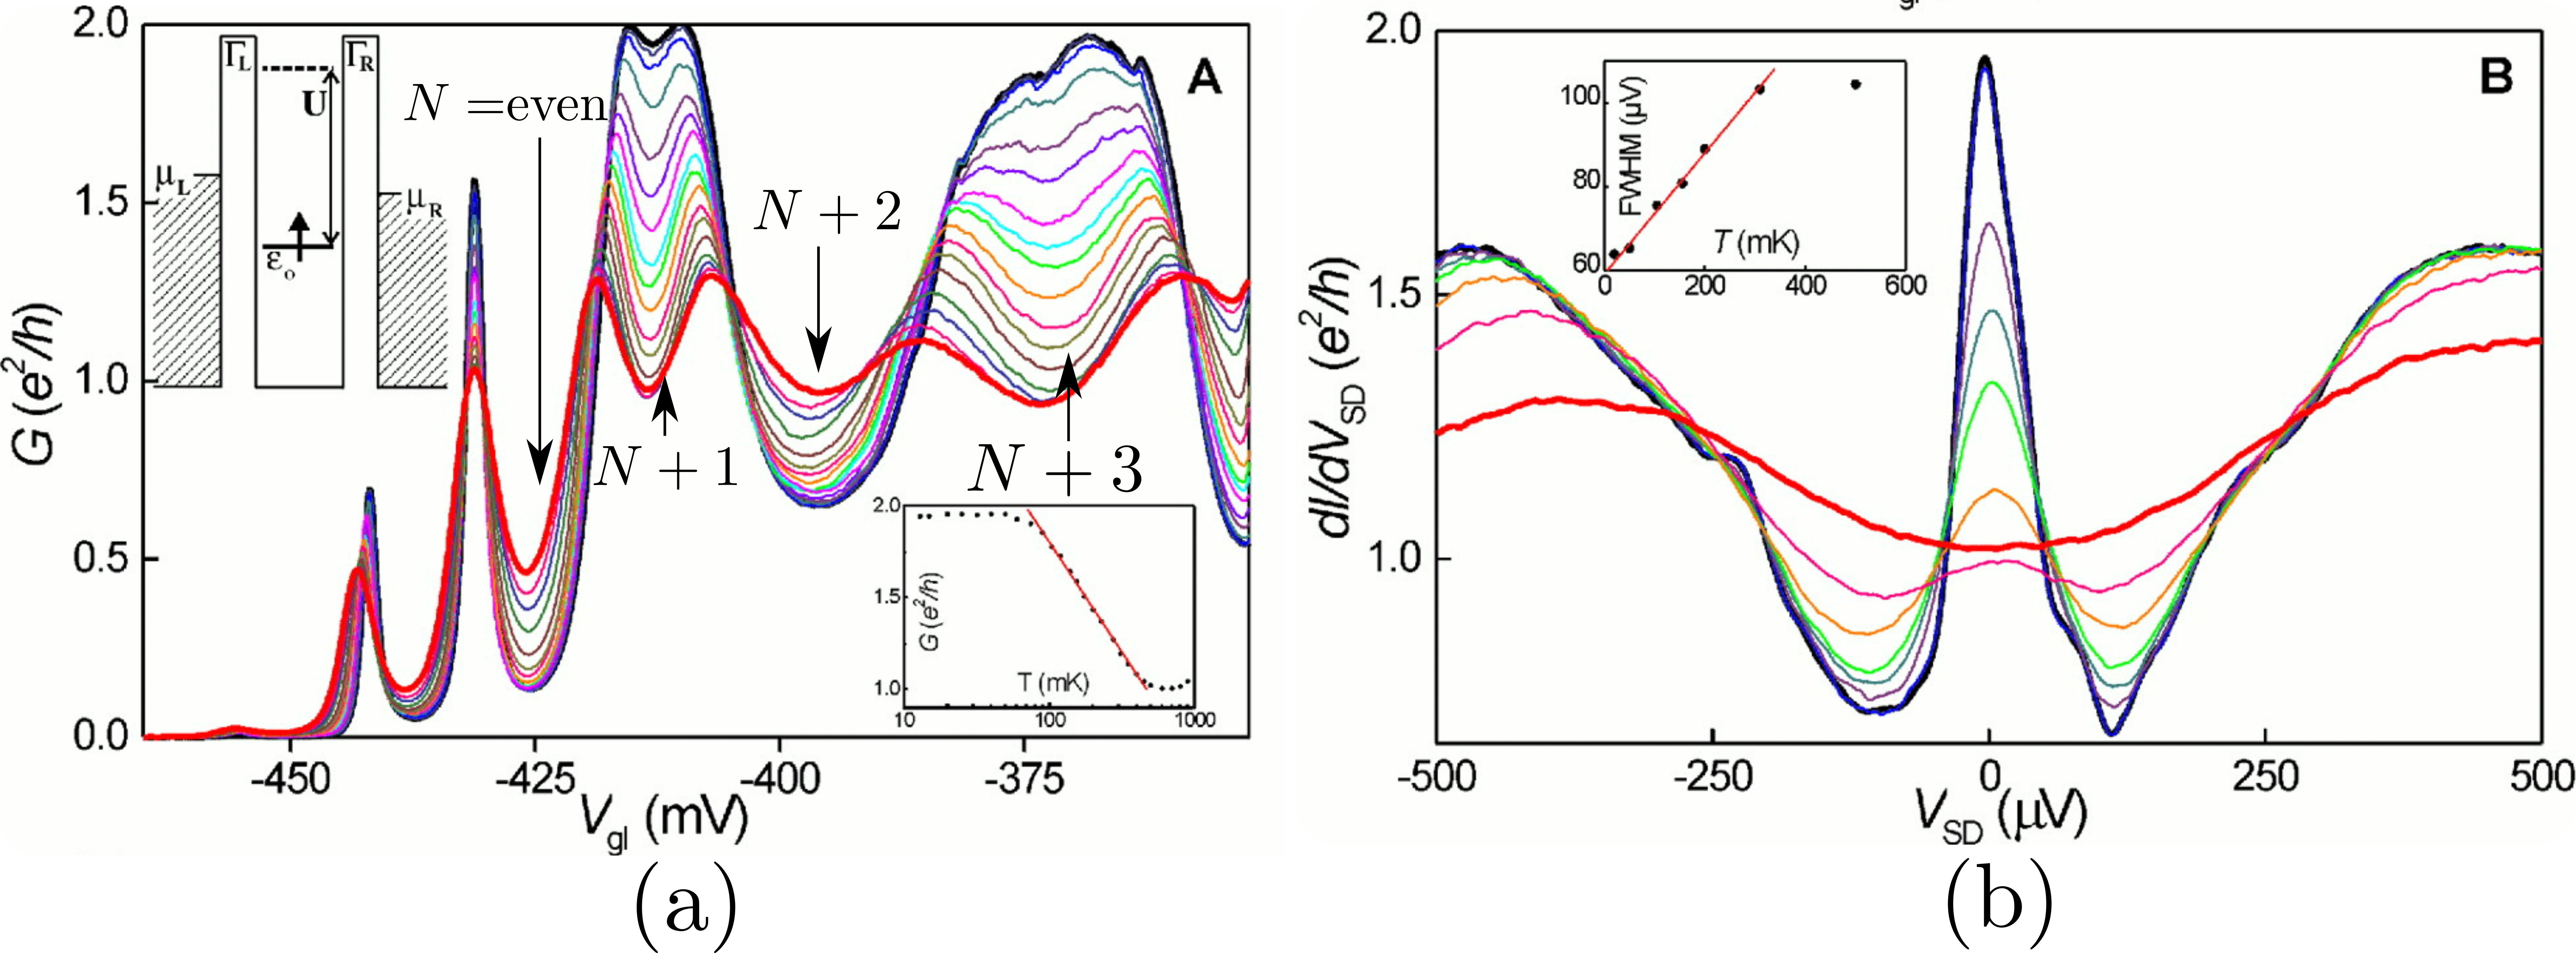
\includegraphics[scale= 0.28]{IMAGES/Preliminars/expKondoQD.png}
  \caption{ \label{fig:ExpKondo} Observation of the Kondo effect in a single electron transistor. Color scale temperatures from 15mk (Black) to 800mk(Red) a) Dependence of the zero bias conductance over the gate voltage. A plato in the conductance peak appears in the odd particle regimes. b) Dependence of the conductance over the gate source drain voltage inside an odd electron regime. A zero bias conductance peak (ZBCP)  of height $\frac{2e^2}{\hbar}$ is observed. This is the Kondo signature.  \protect\Source{\cite{wiel_kondo_2000}}}
\end{figure}


  The problem of magnetic impurities in metals can be treated using the Anderson model in a similar form as the transport in quantum dots. Hence, it is not a surprise that the Kondo Effect could also occur these systems. In 1998 the technological advances allowed the observation of the Kondo effect for the first time in a single electro transistor \cite{goldhaber-gordon_kondo_1998}. When an odd number of electrons is in the QD the last level bellow the Fermi energy is half-occupied and hence the dot can be considered as a magnetic impurity. The unlocalized electrons in the reservoirs then interact with this localized electron. Spin-exchange can occur as it happened with  magnetic impurities in metals. At low temperatures, this magnetic  interaction gives rise to strong quantum correlations that favor the formation of a singlet state between the localized electron and the electrons in the leads. As a result, the zero-bias density of states is increased producing a zero-bias conductance peak \ref{fig:ExpKondo}(b). \\

Note that the physical implications of the Kondo effect  between the case of magnetic impurities in metals and transport through QD are different. The reason for this are the dimensions of the system. While the scattering at 3D systems against magnetic impurities is an obstacle to conduction electrons, the scattering in 0D systems enhances the conductivity of the QD since there is only one scattering direction. 

 As we previously discussed, transport in quantum dots can occur only if there is a state in the middle of the drain and source voltage. The Kondo effect creates a zero bias peak that is present whenever the dot has odd electrons . This explains the zero-bias platoes observed in \ref{fig:ExpKondo}(a). We may think that the new singlet state at the Fermi energy is creating a "channel" that allows quantum transport between both sides of the dot.  
















% The next part of thess preliminaries will be to compute the conductivity
% through the QD as a function of the gate voltage.
% In regular metals the Kondo effect manifests as a drop in conductivity
% under a certain Kondo temperature $(T_{Kondo})$ due to spin- scattering
% between the conduction electrons and the impurities of the material.
% The Anderson models, hence the NRG, are the perfect tools to study
% the physics of impurieties. Thus the computations we previously developed
% in this chapter will provide the right formalism to introduce the
% Kondo physics. This study will be an important part of the prelimiraries
% in the final document. 



%-----------------------------------------------------------

